\chapter{Construcción del algoritmo de simulación}

En este capítulo nos encargaremos de presentar el algoritmo propuesto por Matyka en~\cite{Matyka:Presion}, que es explicado en más detalle en~\cite{Matika:SoftBody}. Este modelo no es más que la unión de los modelos del capítulo anterior. Además definiremos el experimento que deseamos realizar para probar el funcionamieto del modelo.

Más adelante en este mismo capítulo, explicaremos cómo se pueden enfrentar ciertos detalles sobre el algoritmo de Matika.

Primero veremos cómo se puede calcular el volumen de un cuerpo en tres dimensiones, explicaremos como se puede tener una idea general, y por qué para ciertas geometrías del cuerpo, se prestan mejor ciertos algoritmos.

Luego nos enfrentaremos al problema de cómo integrar la ecuación de Newton, con métodos numéricos, analizando dos alternativas, y se presentan las que se consideran las mejores maneras de implementar el integrador en código.

Por último analizaremos el problema más difícil de la implementación: las colisiones. Esto se analiza en dos partes, la manera como se detectan y la respuesta de las mismas.

\section{Diseño del experimento}
\label{descripcion:experimento}
Necesitamos una simulación gráfica (animación) y el principal objetivo será hacer que se \emph{vea} real.

Se quiere modelar un cuerpo neumático. Para hacerlo partimos de un cuerpo flexible y le ponemos un fluido dentro, en este caso el gas, además queremos una manera de probar cómo es la interacción de éste con otros objetos de la escena. 

Con base en esos requerimientos, diseñe la siguiente situación: se modela una caja cerrada, en la cual su cara superior tiene la característica de ser formada como un cuerpo flexible, las otras cinco caras son rígidas. Dentro de esta caja se pone el fluido (gas), de manera que ahora tenemos un cuerpo neumático. Para probar su interacción con otro cuerpo se le deja caer sobre su cara flexible un cuerpo sólido (en este caso una esfera) y se observa el resultado.

Además para poder hacer varios tipos de pruebas se desea que la animación tenga cierta interactividad, es decir que el usuario pueda, en tiempo de ejecución, cambiar algunas opciones tanto de visualización como también algunos parámetros físicos.

Esta simulación es el objetivo principal del trabajo, y el siguiente capítulo está dedicado a cómo se construyó, mientras que en este capítulo se hace énfasis en los detalles teóricos necesarios para escribir el programa.

\section{El algoritmo de simulación de un cuerpo neumático}

Lo primero que debemos de hacer es exponer las condiciones de nuestra simulación de cuerpo flexible. La situación física que deseamos modelar es la de un cuerpo flexible, hueco que contiene un gas. Por ejemplo imagínese un globo, un colchón de aire, la llanta de un automóvil o una burbuja. El comportamiento en el que estamos interesados es en un comportamiento cualitativamente parecido al del fenómeno, es decir que al momento de graficarlo y hacer una animación debe verse \emph{parecido} al sistema real.

El valor de poder graficar de manera realista un modelo como éste, radica en el hecho de que hay muchas cosas que se comportan de manera parecida, y al momento de animar una escena donde hay varios de estos objetos, un modelo físicamente más realista sería muy costoso en tiempo de ejecución.

La forma de atacar este problema será hacerlo con un modelo simple. Imagínese un cuerpo formado por varios puntos unidos entre ellos por resortes.~\footnote{Este modelo es muy socorrido cuando se trata de modelar ropa o tela, se pueden ver ejemplos en el último capítulo de~\cite{FisicaVideojuegos}, que modela una bandera o en~\cite{Vassilev:Ropa} y~\cite{Provot:Ropa}, ambos modelan ropa sobre una persona} Ahora imagínese que a un cuerpo cerrado formado por esta \emph{tela}, le ponemos dentro una fuente de aire, que le ayuda a mantener su forma más o menos constante durante las deformaciones permitidas por los resortes que lo forman; ésa es la idea principal de nuestro modelo.

En la figura~\ref{modelo:fig} podemos ver un pequeño esquema del modelo, en este caso es un hexágono en dos dimensiones. Desde luego, mientras más compleja sea la forma de nuestro modelo, mas difícil será trabajar con él, pero se verá más realista 

\begin{figure}
 \centering
 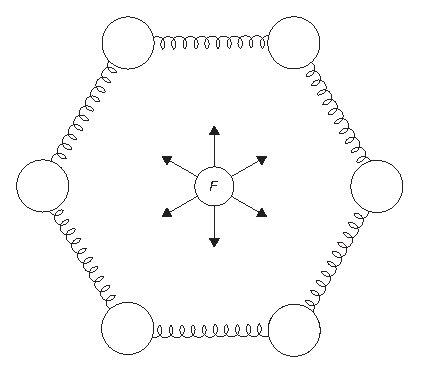
\includegraphics[]{Img/modelo}
 \caption[Diagrama del modelo masa, resorte, y presión]{ 
 Un ejemplo de un modelo de masa resorte, con presión. Se trata de un hexágono cerrado, y $F$ representa la fuerza debida a la presión.
 } \label{modelo:fig}
\end{figure}

\subsection{Esbozo general del algoritmo}
Una vez conocida la idea, nos empezaremos a preguntar en cómo llevarlo a cabo, es decir cómo podemos implementar este modelo en forma de un algoritmo que seamos capaces de codificar en algún lenguaje de programación.


\begin{figure}
 \centering
 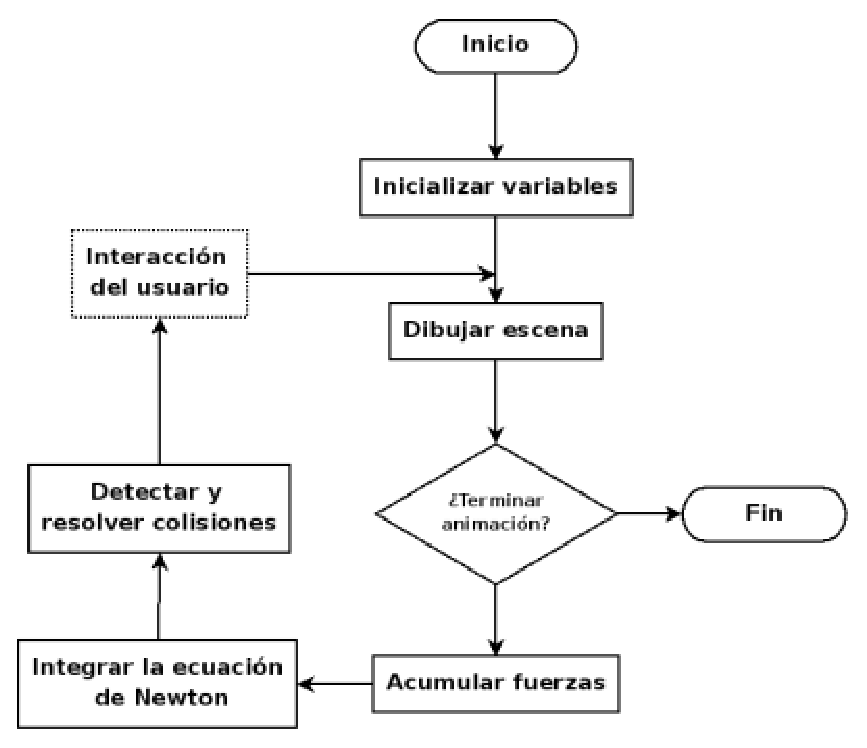
\includegraphics[width=10cm]{Img/diagrama_flujo}
 \caption[Diagrama de flujo de la simulación]{ 
 Este diagrama de flujo muestra, los detalles generales a seguir en una animación de un cuerpo flexible. Para cada paso del algoritmo se pueden tener diferentes estrategias, pero en general este esquema no debe cambiar.
 } \label{diagrama_flujo:fig}
\end{figure}

El diagrama de flujo del algoritmo es el que se muestra en al figura~\ref{diagrama_flujo:fig}, en donde se puede apreciar que sólo se tienen bloques de proceso; cada uno de estos procesos puede ser llevado a cabo de muchas maneras, pero tendrá que ser en este orden, en esta sección veremos con un poco más de detalle cada proceso.

\subsubsection{Inicializar variables}
Lo primero es dar valor a las variables que lo necesiten, me refiero con esto a variables globales, que afectan cómo funciona el programa por el resto de su ejecución. Dentro de estas variables están los parámetros externos del modelo, es decir esos que no pueden ser calculados dentro del programa y que es necesario que se proporcionen por el usuario. Lo parámetros necesarios son $m$ para cada partícula, $g$, $k_d$ y $k_s$ para los resortes, $L$ para cada resorte en particular, y $k_p$ para la acumulación de la fuerza debida a la presión.

Otra cosa que debe hacerse en este paso del algoritmo es poner las condiciones iniciales del modelo, por ejemplo, la posición de cada partícula y la velocidad al momento de iniciar la animación. Y de igual manera con los cuerpos no flexibles que deseemos que interactúen con nuestro modelo, se debe de conocer su posición, si se mueven o no, y cómo van a interactuar con el modelo.

Por último las opciones globales, que afecten a la animación también se deben de obtener aquí, por ejemplo el tamaño del paso $\Delta t$ para mover el modelo, las opciones de los gráficos (si se hará \emph{\foreignlanguage{english}{render}}, o se tratará sólo con el \emph{\foreignlanguage{english}{wireframe}}~\footnote{Cuando sólo se dibujan los bordes de las figuras, como si éstas estuvieran hechas de una malla de alambre se le llama wireframe, cuando dibujamos el área de las figuras y les damos color y efectos de iluminación se dice que se les dio \emph{render}.}) y qué tipo de integrador se ocupará en el modelo. Alguien me podría decir que estos también son parámetros. Y en efecto lo son, quise sin embargo hacer la distinción y llamarlos variables globales, por el hecho de que no se deben al modelo en si, sino más bien a la implementación que cada quien haga del mismo, es decir se deben al programa.

\subsubsection{Dibujar escena}
Esta parte del algoritmo debe ser la encargada de dibujar en la pantalla toda la escena. Para hacer esto debe contar con la información de donde se encuentran cada punto y donde se encuentra cada cosa que queramos dibujar.

Aunque no hay mucho que decir aquí, esta parte es delicada, depende de nuestro conocimiento de las herramientas que vamos a usar para hacer el programa. Con la ayuda de una biblioteca gráfica, en este caso \emph{\foreignlanguage{english}{OpenGL}}, y los datos necesarios guardados de una manera ordenada, como en una estructura de datos, debemos de ser capaces de implementar esta función.

El detalle de la implementación depende del modelo en cuestión, veré a detalle la que yo use. Esto puede ser útil para que alguien que deseé implementar una simulación, se de algunas ideas, pero como ya dije, esta parte depende del fenómeno a modelar, por lo que en cada implementación se debe de hacer un análisis.

\subsubsection{Acumular fuerzas}
Las fuerzas que actúan sobre cada partícula del modelo, se pueden identificar como \emph{externas}, es decir que se deben al medio, o \emph{internas} que se deben al cuerpo en sí. Ejemplos de fuerzas externas son la gravedad, la viscosidad del medio, la resistencia del aire, por mencionar algunas. Ejemplos de las fuerzas internas son por otra parte: los \emph{resortes amortiguadores} y la debida a la presión del gas.

Cualquiera que sea el caso, en este paso debemos de calcular todas las fuerzas, que intervengan en nuestro modelo, y debemos de acumulársela a cada uno de las partículas que lo conforman, es decir, cada partícula debe tener asociada la suma de todas las fuerzas que actúan sobre ella. Recordemos que la fuerza en general es un vector, por lo que la acumulación de la que hablo es una suma vectorial de cada una de las fuerzas.

Los detalles de cómo acomular las fuerzas específicas que ocuparé en la simulación se darán en la siguiente sección y con más a detalle en el resto del capitulo.

\subsubsection{Integrar la ecuación de Newton}
Las fuerzas acomuladas en el paso anterior, junto con la posición y velocidad actuales de la partícula, nos proporcionan (como dice la segunda ley de Newton. Ecuación~\ref{ley:Newton}) el siguiente estado, nos dan la información suficiente para saber la nueva posición y la nueva velocidad de la partícula en cuestión. Conociendo esto para todas las partículas tendremos determinado el estado completo del modelo en el tiempo siguiente.

Como ésta es una ecuación diferencial, debemos de resolverla, o mejor dicho integrarla, para conocer el siguiente estado del sistema, sin embargo como nuestra acomulación de fuerzas fue hecha a partir de muchas fuerzas, todas ellas de naturaleza distinta, no podremos integrar esta ecuación de manera analítica. Por esta razón debemos de recurrir a un método numérico que nos permita aproximar la solución.

Por suerte hay muchísimos métodos numéricos que se ajustan a nuestras necesidades, aquí he decidido presentar a dos de ellos solamente, en la sección dedicada a integrar la ecuación de Newton explicaré a detalle cómo funcionan. De manera general, se puede decir que todos ellos toman como información la posición y velocidad actual de la partícula, el vector fuerza que actúa sobre ella y el instante de tiempo que pasa entre el estado actual y el nuevo estado que queremos calcular (este instante es $\Delta t$). Y después de hacer cálculos con ellos nos devuelven un nuevo estado, en forma de la nueva posición y la nueva velocidad de la partícula.

\subsubsection{Detectar y resolver colisiones}
En este paso debemos analizar qué pasa cuando nuestro modelo choca o interactúa con otros objetos de la escena. Estos otros objetos pueden ser cuerpos rígidos como el piso o flexibles como otro cuerpo de la misma característica del nuestro.

El segundo paso es la respuesta a esta colisión. Este problema es también delicado, pero en general, se va a encargar de ver la partícula que chocó, moverla como respuesta al choque y modificar su estado, es decir su posición y su velocidad. En una sección posterior de este capítulo hablaré con mas detalle y también daré algunas ideas generales.

\subsubsection{Interacción del usuario}
Este paso es opcional, y depende de si deseamos que la simulación tenga una forma de ejecutarse independiente del usuario o si se desea que éste pueda cambiar la simulación en tiempo de ejecución, por ejemplo moviendo alguna partícula, agregando un nuevo cuerpo o modificando algún parámetro de la simulación.

Para enfrentar esto se tiene que recurrir totalmente a la creatividad del programador que vaya a hacer la implementación. Una buena idea es por ejemplo utilizar alguna biblioteca que exista precisamente para este fin (\emph{\foreignlanguage{english}{OpenGL}}, nos proporciona a \emph{\foreignlanguage{english}{glut}}).

\section{El sistema de fuerzas}
Es momento de hacernos unas preguntas: ¿Qué es lo que compone nuestro cuerpo? ¿Qué necesitamos saber para implementar este modelo? La primera pregunta es sencilla: nuestro cuerpo está formado por puntos, que están unidos por resortes, que a su vez se unen para formar las caras. Resumiendo, nuestro cuerpo es un conjunto de caras, que a su vez son un conjunto de resortes, que a su vez son un conjunto de puntos: ¡Nuestro cuerpo está formado por puntos! La respuesta de la segunda interrogante está ligada a la primera, necesitamos saber todo lo que sea necesario para poder acumular fuerza a los puntos, es decir que para cada punto debemos de poder ocupar las ecuaciones~\ref{fuerzaGravedad}~\ref{fuerzaResorte} y \ref{fuerzaGas}.

Ciertamente cada una de estas fuerzas es de naturaleza distinta, la fuerza de gravedad es externa y se puede calcular para cada punto por separado, la de los resortes depende de la posición de cada punto y de sus vecinos a los cuales está conectado por un \emph{resorte-amortiguador} y por último la de presión depende de la cara en la que esté el punto y del volumen total del cuerpo. Podemos resumirlo en el cuadro~\ref{ejemplo:fuerzas}.

\begin{table}
\caption[Resumen de las fuerzas que actúan sobre cada partícula]{Fuerzas a calcular para cada punto y que se necesita saber para hacer los calculos}
\label{ejemplo:fuerzas}
\begin{center}
\begin{tabular} {|p{2cm}|c|p{2cm}|p{7cm}|} \hline
Fuerza & Símbolo &  Parámetros & Datos necesarios \\ \hline
Fuerza de gravedad & $ F_g $ & $g$, $m$ & Ninguno \\ \hline
Fuerza del resorte & $ F_s + F_d $ & $k_s$, $k_d$ & Puntos unidos por el resorte \\
& & & Velocidad y posición de cada punto que une el resorte \\ \hline
Fuerza debida a la Presión & $ F_p $ & $k_p$ & Puntos que forman la cara \\ 
& & & Volumen total del cuerpo \\ 
& & & Area de la cara \\ \hline
\end{tabular}
\end{center}
\end{table}

Para calcular la fuerza de gravedad es necesario que se conozcan dos parámetros, la masa de cada punto $m$, y la constante gravitación $g$. La gravedad debe de acumularse en cada punto.

La fuerza del \emph{resorte amortiguador} es una fuerza interna. Para calcularla  necesitamos recibir dos parámetros: $k_s$ y $k_d$. Luego necesitamos calcular la posición y la velocidad de cada punto, y saber por cada resorte qué puntos está uniendo. Cuando tengamos que acumular esta fuerza recorreremos todos los resortes y por cada resorte calcularemos una fuerza, luego la acomularemos en cada unos de los dos puntos a los que este resorte esté conectado.

Por último, para la fuerza debida a la presión, necesitamos un parámetro externo: $k_p$. Y para poder calcular esta fuerza debemos conocer antes de empezar el volumen total del cuerpo $V$, luego debemos de saber qué puntos pertenecen a cada una de las caras del cuerpo. Para acumular esta fuerza debemos recorrer cada una de las caras que forman el cuerpo, en cada caso calculamos el área de la cara y acumulamos la fuerza $F_p$ que le corresponda en cada uno de los puntos que la forman.

\section{Área, volumen y vectores normales}
Los parámetros necesarios para calcular la fuerza de presión son el volumen total del cuerpo, el área de cada una de las caras, y un vector normal a dicha cara; como ya se dijo, esto depende enteramente de la geometría del cuerpo que se quiera modelar. Sin embargo, esto no quiere decir que no se puedan dar algunas técnicas generales que en alguna medida puedan ser adaptadas a alguna geometría particular. El propósito de esta sección es precisamente el de explicar esas técnicas generales.

\subsection{Cálculo de áreas}
Para calcular el área de un cuerpo geométrico generalmente se calcula el área de cada una de sus caras y después se suman. Empezando por el caso más simple, supongamos que tenemos un triángulo formado por tres puntos, sabemos las coordenadas de cada uno de los puntos, y queremos su área. Supongamos que los puntos son denotados por $P$, $Q$ y $R$. Podemos calcular dos de las aristas del tríangulo si calculamos los vectores que van de $P$ a $Q$ y de $P$ a $R$. Luego podríamos calcular el producto cruz de los dos vectores que acabamos de encontrar y obtener su norma, finalmente la mitad de la norma sería el área del tríangulo que estamos buscando.

$$\overrightarrow{PQ} = Q - P$$
$$\overrightarrow{PR} = R - P$$
$$ A = \frac{1}{2} \vert \overrightarrow{PQ} \times \overrightarrow{PR} \vert$$

Si queremos calcular el área de un cuadrilátero podemos usar la idea anterior y \emph{triangular}, el cuadrilátero en dos partes, supongamos que queremos calcular el área del cuadrilátero formado por los puntos $P$, $Q$, $R$ y $S$, podríamos calcular el área del tríangulo $\triangle PQR$ y luego sumar el área del tríangulo $\triangle SRQ$. Dicho de otra manera:

\begin{eqnarray} 
A_{T} & = & A_{\triangle PQR} + A_{\triangle SRQ} \nonumber \\
A_{T} & = & \frac{1}{2} \vert \overrightarrow{PQ} \times \overrightarrow{PR} \vert \times \frac{1}{2} \vert \overrightarrow{SQ} \times \overrightarrow{SR} \vert \nonumber \\
\label{formulaArea}
A_{T} & = & \frac{1}{2} \left( \vert \overrightarrow{PQ} \times \overrightarrow{PR} \vert + \vert \overrightarrow{SQ} \times \overrightarrow{SR} \vert \right)
\end{eqnarray}

Este resultado de hecho, puede ampliarse aun más con el enunciado siguiente:

Sea $P$ un polígono simple, sin agujeros, dado por la secuencia ordenada de vértices $P_i = (x_i, y_i)$, $i = 1,\ldots,n$, (por ejemplo en el sentido contrario a las agujas del reloj), entonces el área de $P$ es:
$$A(P) = \frac{1}{2}\sum^{n-1}_{i = 1} \det (P_i, P_{i + 1}) + \frac{1}{2} \det (P_n, P_1)$$

Este teorema fue tomado de \cite{GeometriaParaCAD} donde también es demostrado. Con la adecuada combinación de estas técnicas es sencillo ingeniárselas para poder calcular el área de una cara.

\subsection{Cálculo de volúmenes}
Calcular volúmenes es usualmente más complejo que calcular áreas, y por ende casi siempre es computacionalmente costoso, de ahí que además de maneras geométricas de calcular un volumen siempre está la alternativa de aproximar un volumen. De nuevo hay que pensar que queremos lograr con la simulación si rapidez en la ejecución, o apego a la realidad física.

No hay que olvidar también que para todo modelo y sus respectivos parámetros, siempre hay diferentes grados de sensibilidad, por ejemplo en el caso de nuestro modelo el volumen sólo es utilizado para poder determinar la fuerza escalar de la presión, por lo que es un modelo \emph{poco sensible} al cálculo del volumen. Es decir, es válido aproximar en este rubro, sin perder mucha realidad en el modelo.

\subsubsection{Volúmenes aproximados}
Hay varias formas de aproximar el volumen de un cuerpo, una de ellas es con cajas envolventes o \emph{\foreignlanguage{english}{bounding boxes}}, la idea es muy simple se trata de aproximar el volumen de un cuerpo complejo mediante el volumen de un cuerpo simple que lo contenga. Es decir, se aproxima el volumen por medio de poliedros regulares ya sean inscritos o circunscritos, tales que den una buena aproximación del cuerpo cuyo volúmen estamos calculando.

Una forma mas simple es aproximando con un \emph{hexahedro regular} cuyo volumen es $ l \cdot w \cdot h $, o largo por alto por ancho; otra forma geométrica que se usa de manera muy común es el \emph{elipsoide}, cuyo volumen es $ \frac{4\pi}{3} a \cdot   b \cdot  c $, donde $a$, $b$ y $c$, son los largos de sus ejes principales.
\subsubsection{Volúmenes Exactos}
También se pueden tener ciertas técnicas de cálculo de volúmenes exactos mediante la descomposición de un cuerpo en cuerpos simples y calculando después su volumen, que es la técnica que usaremos aquí. Algunos consejos para el cálculo de estos volúmenes son los siguientes.

El volumen de un \emph{paralelepípedo} construido sobre los vectores linealmente independientes $\overrightarrow{OA}$, $\overrightarrow{OB}$ y $\overrightarrow{OC}$ es $V = \vert \det (\overrightarrow{OA}, \overrightarrow{OB}, \overrightarrow{OC} ) \vert $

El volumen del \emph{tetraedro} determinado por los puntos $A_1 = (x_1, y_1, z_1)$, $A_2 = (x_2, y_2, z_2)$, $A_3 = (x_3, y_3, z_3)$ y $A_4 = (x_4, y_4, z_4)$ es:

$$V = \frac{1}{6} \vert \det ( \overrightarrow{A_1 A_2}, \overrightarrow{A_1 A_3}, \overrightarrow{A_1 A_4} ) \vert$$

Como un ampliación a lo hecho en la figura~\ref{vectorArista:fig}, podemos calcular el área del \emph{hexaedro irregular} formado por los ocho puntos $P_1, P_2, \ldots P_8$ tales que los vectores $\overrightarrow{P_1 P_2}$, $\overrightarrow{P_2 P_3}$, $\overrightarrow{P_3 P_4}$ y $\overrightarrow{P_4 P_1}$, formen la tapa superior y los vectores $\overrightarrow{P_1 P_3}$, $\overrightarrow{P_1 P_5}$, $\overrightarrow{P_5 P_7}$ y $\overrightarrow{P_3 P_7}$, formen uno de los lados. Entonces una forma de calcular el volumen es:

\begin{equation}
\label{ecuacionVolumen} 
 V =  \frac{1}{2} \left( \vert \det ( \overrightarrow{P_1 P_2}, \overrightarrow{P_1 P_3}, \overrightarrow{P_1 P_5} ) \vert + \vert \det (\overrightarrow{P_8 P_7}, \overrightarrow{P_8 P_6}, \overrightarrow{P_8 P_4} ) \vert \right) 
\end{equation}

\subsection{Vectores normales}
Dado un plano podemos encontrar un vector que le sea normal, sólo necesitamos dos vectores linealmente independientes que se encuentren en el plano y calculando su producto cruz obtenemos un vector normal, es decir en términos mas simples, si conocemos tres puntos del plano y no son colineales, podemos calcular el vector perpendicular a ese plano.

Matemáticemente: dado el triángulo formado por los puntos $A_1 = (x_1, y_1, z_1)$, $A_2 = (x_2, y_2, z_2)$ y $A_3 = (x_3, y_3, z_3)$, un vector normal a este plano, es el vector $\vec{n}$ que se calcula:

$$ \vec{n} = \overrightarrow{A_1 A_2} \times \overrightarrow{A_1 A_3}$$

Un hecho muy importante es que si queremos calcular el vector normal a una superficie, podemos calcular los vectores normales a cada vértice de ella y luego promediarlos. Esto por increíble que parezca funciona y es de hecho la manera como se hacen los cálculos de iluminación en la mayoría de los programas de CAD y de simulación gráfica.

Es decir, si tenemos el polígono de $n$ lados, formado por los puntos $P_1, P_2, \ldots, P_n$, ordenados de alguna manera, por ejemplo en sentido contrario a las manecillas del reloj, y queremos el vector normal a este polígono $\vec{n}$, calculamos los vectores $ v_1, v_2, \ldots , v_n $, de la forma $v_i = \overrightarrow{P_i P_{i + 1}} \times \overrightarrow{P_i P_{i + 1}} $ para $i = 2, \ldots, n$ y $v_1 = \overrightarrow{P_1 P_2} \times \overrightarrow{P_1 P_n}$, y luego el vector normal $\vec{n}$ es:

\begin{equation}
\label{formulaVecNormal} 
\vec{n} = \frac{1}{n} \sum_{i=1}^{n} v_i
\end{equation}

Este hecho es fundamental para nuestros cálculos, tanto de la fuerza debida a la presión, como para la iluminación en el render. Una demostración se puede encontrar en \cite{GeometriaParaCAD}.

\section{Integrar la ecuación de Newton}
Desde que hay modelos físicos, ha habido interés en la solución numérica de ciertos problemas para los que se sabía de antemano que una solución existía, pero no se contaban con métodos adecuados para encontrarla. Es por esta razón que nace el análisis numérico, sin embrago no fue hasta que se popularizó el uso de las computadoras que este campo tomó más importancia.

Dentro del análisis numérico, es de nuestro interés la solución numérica de ecuaciones diferenciales. El problema comienza con una ecuación de primer orden con condición inicial y que cumple las condiciones de existencia y unicidad.

Actualmente hay muchas maneras de atacar estos problemas, es decir muchas familias de métodos. Por familia quiero decir cuando alguien propone un método y llega otra persona más y le hace correcciones, ahora hay dos métodos pero en escencia funcionan con la misma idea, por eso son dos métodos de la misma familia.

El primer método para obtener una aproximación numérica de la solución de una ecuación diferencial es el método de Euler, y desde entonces se han propuesto muchísimos métodos e ideas más. El cuadro~\ref{historia:metodos} es una línea del tiempo que tiene algunos de los acontecimientos más importantes del desarrollo de esta disciplina.

\begin{table}
\caption[Evolución histórica de los métodos numéricos]{Una línea de tiempo que muestra algunos de los acontecimientos mas importantes para la solución numérica de ecuaciones diferenciales}
\label{historia:metodos}
\begin{center}
\begin{tabular} {|c|p{12cm}|} \hline
Año & Evento \\ \hline
1768 & Leonhard Euler publica su método, el primero en la historia \\
1824 & Agustin Cauchy demuestra la convergencia del método de Euler, emplea el método de Euler implícito \\
1855 & En una carta escrita por John F. Bashforth, se mencionan por primera vez los metodos de pasos multiples de Couch Adams \\
1895 & Carl Runge publica el primer método de Runge Kutta \\ 
1905 & Martin Kutta describe el popular método de Runge Kutta de orden cuatro \\ 
1910 & Lewis Fry Richardson anuncia su método de extrapolación. \\
1952 & Charles F. Curtiss y Joseph Oakland Hirschfelder acuñan el término \emph{\foreignlanguage{english}{stiff equations}}. \\
1967 & Loup Verlet publica su método, especialmente enfocado a la mecánica de partículas \\ \hline
\end{tabular}
\end{center}
\end{table}

En escencia estos métodos se encargan de resolver la ecuacion diferencial de la forma:
\begin{eqnarray}
 \frac{dy}{dt} & = &f(t,y) \nonumber \\
 y(t_0) & = & y_0 \label{condicion:inicial}
\end{eqnarray}

Y para hacerlo toman la condición inicial~\ref{condicion:inicial}, como el primer valor de la solución, con ella calculan un valor aproximado para la solución $y(t)$ en el tiempo $t = t_0 + \Delta t$. Ahora este nuevo punto de la solución lo llamamos $y_{n}$ y nos ayuda a encontrar un nuevo punto dando otro paso hacia adelante en el tiempo $t = y_0 + 2\Delta t$
Y así sucesivamente, de manera que la salida de nuestro método son una colección de parejas $(t + n \Delta t, y(t + n \Delta t) )$ la primera de ellas es la condición inicial, y de ahí en adelante se trata de aproximaciones de la solución.

Sin embargo nosotros no queremos resolver una ecuación como ésta, deseamos resolver la ecuación~\ref{ley:Newton}, que es una ecuación diferencial de segundo orden. Para poder adaptar este problema al método se propone un cambio de variable $\frac{dx}{dt} = v(t)$, por lo que el problema se transforma en resolver un sistema de dos ecuaciones diferenciales.

\begin{eqnarray}
\frac{dv}{dt} & = & \frac{1}{m} F(x, v, t) \nonumber \\
\frac{dx}{dt} & = & v(t) \nonumber \\
v(0) & = & v_0 \nonumber \\
x(0) & = & x_0 \nonumber
\end{eqnarray}

Los métodos siguientes entonces supondrán que sabemos la velocidad y la posición de la partícula en el tiempo $t$, así como la fuerza que actúa sobre ella en este tiempo, con esta última podremos calcular la posición y la velocidad de la partícula en un tiempo posterior $t + \Delta d$.

\subsection{El método de Euler}
Este método fue el primero de todos, de ahí que también sea el más simple, sin embargo aún tiene algunas ventajas el usarlo. Básicamente el método de Euler nos dice que si tenemos una ecuación de la forma:
$$y'(t) = f(t, y)$$
Con una condición inicial de la forma $y(0)=y_0$.

Entonces podemos aproximar el siguiente punto de la solución con la siguiente fórmula de recurrencia:

$$y_{n+1} = y_n + hf(t_n, y_n)$$

En donde $h$ representa el tamaño del paso en el tiempo hacia adelante es decir $h = \Delta t$.

El método de Euler se puede generalizar para sistemas de ecuaciones diferenciales de tamaño $n$. Estas generalizaciones se pueden ver en casi cualquier libro de Ecuaciones y en cualquier libro de análisis numérico. Aquí sólo daré las fórmulas de recurrencia para el caso de $n=2$ por ser el que estamos interesados en resolver.

Dado el sistema:
\begin{eqnarray}
x'(t) & = & f(t, x, y) \nonumber \\
y'(t) & = & g(t, x, y)
\label{sistema:general}
\end{eqnarray}
Con las condiciones iniciales:

\begin{eqnarray}
x(t_0) & = & x_0 \nonumber \\
y(t_0) & = & y_0
\label{condiciones:general}
\end{eqnarray}

Entonces la solución se puede aproximar con las siguientes fórmulas de recurrencia:
$$x_{n+1} = x_n + hf(t_n, x_n, y_n)$$
$$y_{n+1} = y_n + hg(t_n, x_n, y_n)$$

Ahora vamos a poner nuestro sistema de manera que podamos ocupar estas fórmulas para resolverlo:
\begin{eqnarray}
v'(t) & = & \frac{1}{m}F(t, x, v) \nonumber \\
x'(t) & = & v(t, x, v)
\label{sistema:particular}
\end{eqnarray}

Y nuestras condiciones iniciales son:
\begin{eqnarray}
v(t_0) = v_0 \nonumber \\
x(t_0) = x_0
\label{condiciones:particular}
\end{eqnarray}

Por lo tanto para resolver nuestro sistema con el método de Euler se tiene:

\begin{eqnarray}
v_{n+1} & = & v_n + \frac{h}{m}F(t_n, x_n, v_n)\nonumber \\
x_{n+1} & = & x_n + hv_{n + 1}
\label{formulas:Euler}
\end{eqnarray}

\subsubsection{El error del método de Euler}
Como en todo procedimiento numérico, en el método de Euler se tiene un error, el cual puede encontrarse para nuestro caso por medio de la expansión en la serie de Taylor para la función que determina la posición de una partícula.

$$x_{n+1}  =  x_n + hv_n$$
$$x(t_0 + h) = x(t_0) + h v(t_0)$$

Pero sabemos que la serie de Taylor de la trayectoria de una partícula es:

$$x(t_0 + h) = x(t_0) + h x'(t_0) + \frac{1}{2}h^2x''(t_0) + O(h^3)$$

Entonces el error en el método de Euler está dado por la diferencia de ambas expresiones es decir:

$$-\frac{1}{2}h^2x''(t_0) + O(h^3)$$

Este error es el error de truncamiento, o debido al método en sí. Al momento de implementarlo existe también un error por redondeo, que es debido a que las computadoras operan con un número finito de decimales, sin embargo este error es difícil de estimar y sale del alcance de mi investigación. De aquí en adelante cuando me refiera al error de un método numérico siempre me referiré al \emph{error por truncamiento}.

\subsubsection{Ventajas y desventajas del método de Euler}

Como todo algortimo este método presenta ventajas y desventajas, éstas se deben tanto al método como a su implementacion en este modelo. Aquí listaré algunas de ellas.

Ventajas:
\begin{itemize}
\item Se puede implementar fácilmente.
\item Se puede integrar partícula por partícula, dado que sólo requiere de una evaluación de $F$.
\item Es rápido de ejecutarse.
\end{itemize}

Desventajas:
\begin{itemize}
\item Tiende a \emph{explotar} rápidamente.
\item Su error es alto.
\item Es muy sensible a las variaciones pequeñas, por lo que tarda en estabilizarse.
\end{itemize}

\subsection{El método de Runge Kutta}
Supongamos que se tiene una ecuación de la forma
$$y'(t) = f(t, y)$$
Con su respectiva condición inicial de la forma $y(0)=y_0$.

El método de Runge y Kutta nos dice que la solución en el siguiente paso de tiempo puede aproximarse con la siguiente fórmula de recurrencia:
$$y_{n+1} = y_n + \frac{h \left(k_{n1} + 2k_{n2} + 2k_{n3} + k_{n4} \right)}{6} $$
 
En donde $h$ representa el tamaño del paso en el tiempo que se desee aproximar y los coeficientes $k_{n1}$, $k_{n2}$, $k_{n3}$, $k_{n4}$ se pueden calcular de la siguiente manera:

\begin{eqnarray}
k_{n1} & = & f(t_n, y_n) \nonumber \\
k_{n2} & = & f(t_n + \frac{h}{2}, y_n + \frac{h}{2} k_{n1}) \nonumber \\
k_{n3} & = & f(t_n + \frac{h}{2}, y_n + \frac{h}{2} k_{n2}) \nonumber \\
k_{n4} & = & f(t_n + h, y_n + hk_{n3}) \nonumber
\end{eqnarray}

Al igual que en el método de Euler, existe una generalización del método de Runge Kutta para poderse ocupar con sistemas de ecuaciones de primer orden. En casi cualquier libro de ecuaciones se pueden ver estas fórmulas (por ejemplo en~\cite{Blanchard:Ecuaciones}); aquí solo pongo el caso $n=2$ porque es el que voy a ocupar en el modelo.

Supongamos que tenemos de nuevo el sistema~\ref{sistema:general}, sujeto a~\ref{condiciones:general}. Podemos aproximar una solución usando el método de Ruge Kutta con la siguiente fórmula de recurrencia, suponiendo que queremos ir de $t_n$ a $t_{n+1}$.

\begin{eqnarray}
x_{n+1} & = & x_n + \frac{h(k_{n1} + 2k_{n2} + 2k_{n3} + k_{n4})}{6} \nonumber \\
y_{n+1} & = & y_n + \frac{h(l_{n1} + 2l_{n2} + 2l_{n3} + l_{n4}))}{6} \nonumber
\end{eqnarray}

Aquí podemos apreciar que ahora tenemos que encontrar cuatro ponderadores, los $k_i$ y $l_i$ significa que tenemos mas cálculos por hacer. Los valores de los ponderadores se calculan con las siguientes fórmulas.

\begin{eqnarray}
k_{n1} & = & f(t_n, x_n, y_n) \nonumber \\
k_{n2} & = & f(t_n + \frac{h}{2}, x_n + \frac{h}{2} k_{n1}, y_n + \frac{h}{2}l_{n1}) \nonumber \\
k_{n3} & = & f(t_n + \frac{h}{2}, x_n + \frac{h}{2} k_{n2}, y_n + \frac{h}{2}l_{n2}) \nonumber \\
k_{n4} & = & f(t_n + h, x_n + hk_{n3}, y_n + hl_{n3}) \nonumber
\end{eqnarray}

y

\begin{eqnarray}
l_{n1} & = & g(t_n, x_n, y_n) \nonumber \\
l_{n2} & = & g(t_n + \frac{h}{2}, x_n + \frac{h}{2} k_{n1}, y_n + \frac{h}{2}l_{n1}) \nonumber \\
l_{n3} & = & g(t_n + \frac{h}{2}, x_n + \frac{h}{2} k_{n2}, y_n + \frac{h}{2}l_{n2}) \nonumber \\
l_{n4} & = & g(t_n + h, x_n + hk_{n3}, y_n + hl_{n3}) \nonumber
\end{eqnarray}


El método de Runge Kutta, es mucho más exacto que el método de Euler, de hecho se puede apreciar que el método de Euler, aproxima el siguiente paso con el valor de una pendiente, en cambio el método de Runge Kutta aproxima el siguiente paso con el valor de cuatro pendientes ponderadas, cada una calculada con la aproximación de la anterior.

Supongamos que se tiene de nuevo~\ref{sistema:particular} sujeto a las condiciones~\ref{condiciones:particular}, entonces el metodo de Runge Kutta toma la siguiente forma:

\begin{eqnarray}
v_{n+1} & = & v_n + \frac{h}{6}(k_{n1} + 2k_{n2} + 2k_{n3} + k_{n4}) \nonumber \\
x_{n+1} & = & x_n + \frac{h}{6}(l_{n1} + 2l_{n2} + 2l_{n3} + l_{n4})
\label{formulas:RK4}
\end{eqnarray}

Y los ponderadores se pueden calcular de la siguiente manera:

\begin{eqnarray}
k_{n1} & = & \frac{1}{m}F(t_n, x_n, v_n) \nonumber \\
l_{n1} & = & v_n \nonumber \\
k_{n2} & = & \frac{1}{m}F(t_n + \frac{h}{2}, \, x_n + \frac{h}{2}k_{n1}, \, v_n + \frac{h}{2}l_{n1}) \nonumber \\
l_{n2} & = & v_n + \frac{h}{2}k_{n1} \nonumber \\
k_{n3} & = & \frac{1}{m}F(t_n + \frac{h}{2}, \, x_n + \frac{h}{2}k_{n2}, \, v_n + \frac{h}{2}l_{n2}) \nonumber \\
l_{n3} & = & v_n + \frac{h}{2}k_{n2} \nonumber \\
k_{n4} & = & \frac{1}{m}F(t_n + h, \, x_n +hk_{n2}, \, v_n + hl_{n2}) \nonumber \\
l_{n4} & = & v_n + hk_{n3}
\label{ponderadores:RK4}
\end{eqnarray}

\subsubsection{El error del método de Rungue Kutta}
Se puede demostrar por medios algebraicos y de la misma manera que se empleó con el método de Euler que el método de Runge Kutta tiene un error del orden de $O(h^5)$. Es decir si partimos el intervalo $h$ por la mitad, y damos el doble de pasos el error por truncamiento disminuye en un orden de 16 veces (es decir $\left( \frac{h}{2} \right)^4$, como el error es del orden de $O(h^5)$ se hace $h^4$ veces más exacto).

\subsubsection{Ventajas y desventajas del metodo de Runge Kutta}
Como se puede leer en la bibliografía, el método de Euler y el método de Runge Kutta dependen del tamaño del paso $h$, y se hacen más exactos mientras el paso es más pequeño, pero también se hacen más cálculos, por lo que aumenta la fuente del otro tipo de error, el error por redondeo. Se acepta de manera general, que de este tipo de métodos, aquel que optimiza esta situación es el método de Runge Kutta de cuarto orden, el método que acabamos de presentar.

Algunas de las ventajas y desventajas para el método de Runge Kutta son las siguientes.

Ventajas
\begin{itemize}
\item Es el método estándar más recomendado y no es tan difícil de implementar (métodos más exactos son considerablemente más difíciles de implementar).
\item Es recomendado por muchos autores y por lo tanto hay mucha documentación.
\item Es rápido de ejecutarse, (Más lento que el Euler, pero para efectos de la animación la diferencia no es apreciable).
\item Es un método muy estable, es muy difícil que explote.
\end{itemize}

Desventajas
\begin{itemize}
\item A diferencia de Euler, requiere de muchas evaluaciones de la función en diferentes puntos (lo que para nosotros significa calcular muchas veces la fuerza sobre la partícula).
\item Las partículas no se pueden integrar por separado, tendrán que integrarse juntas. (todas las que conforman el cuerpo en un solo paso).
\end{itemize}

\section{Cómo enfrentar la colisión de los cuerpos}
Por colisión de los cuerpos entenderemos la manera como lidiar cuando dos cuerpos dentro de la escena quedan en contacto uno con el otro. Desde nuestro punto de vista esta respuesta se divide en dos pasos: la detección de la colisión y la respuesta a la colisión.
La detección es totalmente un problema geométrico, consiste en que a partir de la información que tenemos de los cuerpos y de la colisión podemos determinar al punto de la colisión y un vector normal a ese punto, este problema es totalmente dependiente de la forma de los cuerpos. Por el otro lado la respuesta a la colisión es un problema físico y generalmente es más sencillo debido que ya existen algoritmos bien definidos para responder a las colisiones y son independientes de la geometría, es decir son algoritmos generales.

\subsection{La detección de las colisiones}
Como ya se dijo antes la detección de las colisiones es uno de los problemas más complejos que nos podemos enfrentar al hacer una animación. Básicamente debemos de poder hacer dos cosas aquí: uno, detectar la colisión, es decir mediante una prueba rápida saber si los cuerpos de nuestra escena entraron en contacto, y después ver si podemos determinar un vector normal al punto (o superficie en 3D) de colisión.

Hay básicamente dos tipos de estrategias para resolver este problema, una es por medio de un \foreignlanguage{english}{\emph{bounding volume}}, que se trata de darle la vuelta al problema con una aproximación y otra es por medios estrictamente geométricos es decir tratar de dividir tus cuerpos en figuras de formas elementales, como esferas o paralelepípedos para los cuales las detección es un poco más sencilla.

\subsubsection{Un \foreignlanguage{english}{\emph{bounding volume}}}
Básicamente se trata de imaginar que hay un envolvente de nuestro objeto y este envolvente tiene una forma más sencilla, entonces al probar por la colisión se prueba con el envolvente no con el objeto. Esto tiene la enorme desventaja de ser una aproximación, por lo que la animación se vera un poco saltada, sin embargo una cuidadosa elección del objeto envolvente hará que este efecto sea mínimo.

Objetos como las elipses, los paralelepípedos y los cilindros son buenos objetos para ser un \foreignlanguage{english}{\emph{bounding volume}}, porque la detección de la colisión es sencilla.

Por ejemplo, en una esfera podemos determinar si un punto esta dentro de ella con tan sólo comparar el cuadrado de su distancia con respecto al centro de la esfera, con el cuadrado del radio. 

Un cilindro con el eje vertical alineado con el eje de la escena es también muy usado. Si queremos saber si dos objetos contenidos en un cilindro, por ejemplo en un videojuego dos personajes caminando, chocan, sólo debemos ver si la proyección de los ejes principales de los cilindros sobre el eje de la escena (líneas rectas) se interceptan y además las proyecciones de los dos cilindros con el plano $XZ$ (dos círculos) también se intersecan.

Un paralelepípedo o rectángulo, o \foreignlanguage{english}{\emph{bounding box}}, también se usa mucho, por ejemplo cuando la geometría de los objetos hace a la esfera una mala elección, por ejemplo al ver si dos coches chocan en un juego de carreras el rectángulo es una elección mas sabia.

Un rectángulo usado como \foreignlanguage{english}{\emph{bounding box}} generalmente se alinea con las coordenadas del mundo, para así hacer las pruebas de detección triviales, si  por el contrario el rectángulo es alineado con las coordenadas del objeto y este tiene la capacidad de rotar, cada vez que lo haga se necesita volver a calcular el  \foreignlanguage{english}{\emph{bounding box}}.
\subsubsection{Uniendo diferentes geometrías}
Una manera más exacta de predecir si dos objetos de una escena están en colisión, es descomponer la forma completa de un objeto en varios objetos pequeños, y luego probar contra todos los objetos que componen el cuerpo si es que existió la colisión. Por ejemplo, en el caso de la simulación del cuerpo flexible se podría pensar como que cada partícula que forma el cuerpo es un objeto y luego probar la colisión contra todas las partículas que forman el cuerpo flexible.

Esta técnica es bastante más cara, tanto de implementar como de ejecutarse, sin embargo, da resultados visiblemente más acertados, por ejemplo en un juego de lucha libre, donde la interacción de los luchadores debe de ser bastante creíble, se recomendaría usar este tipo de colisiones.

\subsection{La respuesta de las colisiones}

Como ya habíamos dicho, el trabajo difícil y dependiente de la animación está en la detección de las colisiones, y la respuesta a las colisiones es totalmente física. Para empezar las colisiones se dividen en dos: elásticas e inelásticas. La implementación de ambas no se diferencia mucho, aunque sí son diferentes en concepto.

Básicamente en un algoritmo de respuesta de colisiones, se suministran las posiciones y las velocidades de los dos objetos que coliden, más un vector normal al punto de colisión de los dos objetos, o plano normal en el caso de tres dimensiones. Desde luego que hay dos vectores que cumplen con esa condición, cualquiera de ellos nos servirá siempre y cuando sepamos cual de ellos es el que tenemos. Ya con esta información debemos ser capaces de responder con dos cosas: una nueva posición de los objetos y una nueva velocidad.

En la figura~\ref{colision:fig} se ven los diferentes pasos de la respuesta a la colisión de dos círculos.
\begin{figure}
 \centering
 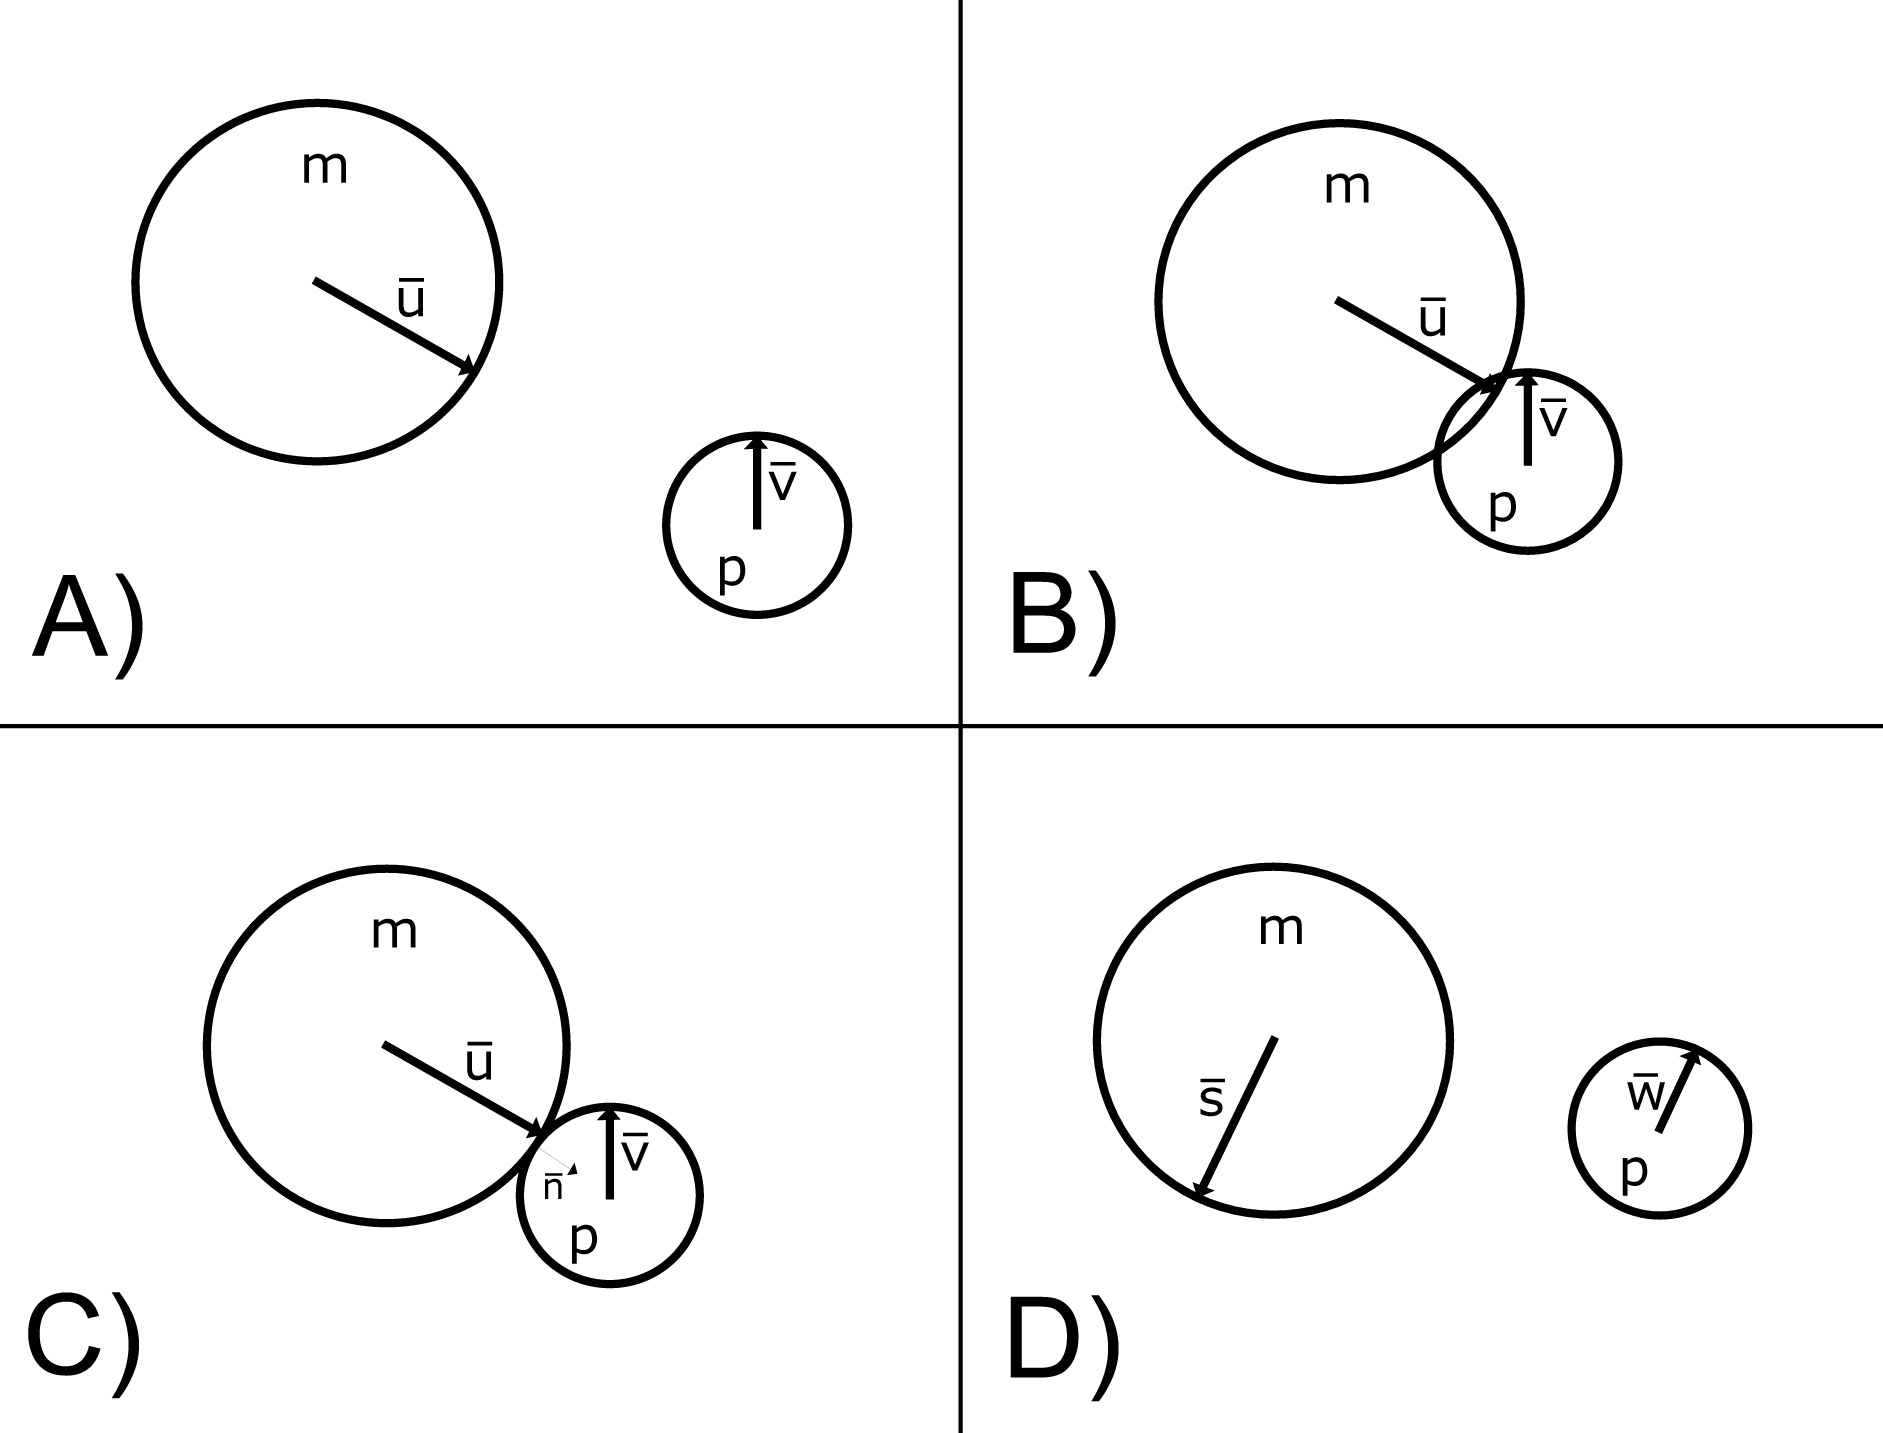
\includegraphics[]{Img/colisiones}
 \caption[Colisión elástica]{A) La situación justo antes de que ocurra la colisión. B)La situación en el momento en que se detecta la colisión. C)La respuesta a la colisión. D)Las velocidades ajustadas después de la colisión} 
 \label{colision:fig}
\end{figure}

\subsubsection{Separar un vector en componentes normal y tangencial}
Antes de explicar la forma en que se responden las colisiones quiero hacer énfasis en la manera como separa un vector en componentes ortogonales (figura \ref{comVec:fig}), porque es necesario hacerlo en la respuesta a las colisiones.

Para separar a un vector cualquiera $\vec{v}$ en dos componentes: uno normal $\vec{v_n}$, y otro tangencial $\vec{v_t}$ respecto a un vector normal $\vec{n}$, se hace uso de las siguientes fórmula:

\begin{eqnarray}
\vec{v_n} & = &\frac{(\vec{v} \cdot \vec{n})}{|\vec{n}|} \frac{\vec{n}}{|\vec{n}|} \nonumber \\
\vec{v_t} & = & \vec{v} - \vec{v_n} \nonumber
\end{eqnarray}

Como en los cálculos de detección de colisiones es común que tengamos un vector normal $\vec{n}$, tal que: $|\vec{n}| = 1$, las fórmulas anteriores se simplifican aun más siendo la forma más usada la siguiente\footnote{Las fórmulas~\ref{eq:sepVector}, se encuentran mal escritas en~\cite{BaraffWitkin:Coursenotes}, y esta fue una de las razones que más me retrasó al momento de hacer este trabajo.}:

\begin{eqnarray}
\vec{v_n} & = &(\vec{v} \cdot \vec{n}) \vec{n} \nonumber \\
\vec{v_t} & = & \vec{v} - \vec{v_n}
\label{eq:sepVector} 
\end{eqnarray}

\subsubsection{Colisiones elásticas}

Una colisión elástica es aquella donde el momento y la energía de los objetos, se conservan después de la colisión; son una abstracción que nunca sucede en la vida real. Aun las colisiones en el espacio exterior son inelásticas aunque están muy cerca de no serlo~\cite{FisicaMatematicasVideojuegos}, pero nos sirven bastante para entender el fenómeno, y en algunos casos son suficientes. Por ejemplo, pensemos que estamos modelando un juego de billar en 2D una colisión elástica es suficiente.

Supongamos que se tienen dos cuerpos $A$ y $B$, las formas no importan, y sabemos, gracias a un algoritmo de detección de las colisiones, que están en colisión y  un vector normal $\vec{n}$ a la superficie de colisión. Suponemos que este vector apunta del cuerpo $A$ al cuerpo $B$ y que es también un vector unitario.

Suponemos también que conocemos todas las propiedades de los cuerpos, es decir su masa, su velocidad y su posición.

Queremos determinar una nueva posición y una nueva velocidad para los objetos como resultado de la colisión entre ellos. Esto se resumen el el cuadro~\ref{condiciones:Colision}.
\begin{table}
\caption{Condiciones de la respuesta a las colisiones}
\label{condiciones:Colision}
\begin{center}
\begin{tabular} {|c|c|c|} \hline
Objeto & Información conocida & Información por determinar \\ \hline
$A$ & Masa $m$, Velocidad $\vec{u}$ & Velocidad ajustada $\vec{s}$ \\
$B$ & Masa $p$, Velocidad $\vec{v}$ & Velocidad ajustada $\vec{w}$ \\ \hline
\end{tabular}
\end{center}
\end{table}

Para entender el porqué de la respuesta a la colisión, es necesario seguir los siguientes pasos\footnote{Esta es una reproducción del procedimiento mostrado en~\cite{FisicaMatematicasVideojuegos} con mi nomenclatura}. Primero vamos por el caso más simple: dos objetos $A$ y $B$, con velocidades $\vec{u}$ y $\vec{v}$ respectivamente chocan, como respuesta a la colisión las velocidades de ambos objetos cambian a $\vec{s}$ y $\vec{w}$. Ver la figura~\ref{colision:fig}.

Suponemos que: $\vec{v} = 0$. Es decir el cuerpo $B$ no se mueve, está detenido esperando la colisión del cuerpo $A$. Sabemos que tenemos un vector $\vec{n}$ normal al plano de colisión. Con este vector podemos dividir los demás vectores en una parte normal al plano y otra tangencial  (figura~\ref{comVec:fig}), es decir:

\begin{figure}
 \centering
 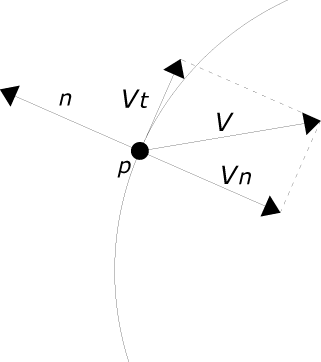
\includegraphics[width=5cm]{Img/vector_componente}
 \caption[Separar componente tangencial y normal de un vector]{ 
 El vector $V$ se separa con respecto a $n$ en dos vectores uno normal $V_n$, y uno tangencial $V_t$ 
 } \label{comVec:fig}
\end{figure}

\begin{eqnarray}
 \vec{u} & = & \vec{u_t} + \vec{u_n} \nonumber \\
 \vec{v} & = & \vec{v_t} + \vec{v_n} \nonumber \\
 \vec{s} & = & \vec{s_t} + \vec{s_n} \nonumber \\
 \vec{w} & = & \vec{w_t} + \vec{w_n} \nonumber
\end{eqnarray}

Ahora veamos que es lo qué sabemos de antemano por la forma como planteamos las condiciones del problema: sabemos que: $\vec{u_t} = \vec{s_t}$ y $\vec{v_t} = \vec{w_t} = 0$, porque esperaríamos que las velocidades sólo se vieran afectadas en su componente normal y porque sabemos que el objeto $B$ estaba inicialmente en reposo. Así que lo único que necesitamos saber es $\vec{s_n}$ y $\vec{w_n}$.

Se sabe también que, como la colisión es elástica, debe de obedecer la ley de la conservación de la energía y la la ley de la conservación de momento.

\begin{equation}
m \bar{u_n} = m \bar{s_n} + p \bar{w_n}
\label{eq:momento}
\end{equation}

\begin{equation}
\frac{1}{2} m \bar{u}^2 = \frac{1}{2} m \bar{s}^2 + \frac{1}{2} p \bar{w}^2
\label{eq:energia}
\end{equation}

Así que tenemos justo las condiciones necesarias para encontrar una solución, pues tenemos dos valores por determinar y dos ecuaciones que las relacionan. Para encontrar la solución hacemos un cambio de variable $r = \frac{m}{p}$. Luego despejamos de la ecuación~\ref{eq:momento} a $\bar{w_n}$, y lo sustituimos en~\ref{eq:energia} y obtenemos el valor de $\bar{s_n}$. En realidad se obtienen dos valores $\bar{s_n} = \bar{u_n}$ y $\bar{s_n} = \bar{u_n} \frac{r-1}{r+1}$, tomamos el segundo (el primero corresponde a la condición inicial, por que las colisiones elásticas son reversibles en el tiempo), y lo sustituimos de nueva en~\ref{eq:momento} para obtener el valor de $\bar{w_n} = \frac{2 r \bar{u_n}}{r + 1}$.

Con esto se tiene todo lo necesario  para resolver una colisión elástica con uno de los dos objetos en reposo. Podemos utilizar el siguiente pseudocódigo:

\begin{enumerate}
 \item $r = \frac{m}{p}$
 \item $\bar{u_n} = parteNormal(\vec{u}, \vec{n})$
 \item $\bar{u_t} = \bar{u} - \bar{u_n}$
 \item $\bar{s_n} = \bar{u_n} \left( \frac{r - 1}{r + 1} \right) $
 \item $\bar{w_n} = \bar{u_n} \left( \frac{2r}{r + 1} \right) $
 \item $\bar{s} = \bar{u_t} + \bar{s_n}$
 \item $\bar{w} = \bar{w_n}$
\end{enumerate}
En donde la función \verb|parteNormal|, es una función que recibe un vector $\vec{u}$ y un vector $\vec{n}$, devuelve la parte normal de $\vec{u}$ con respecto a $\vec{n}$. Es decir nos sirve para partir al vector $\vec{u}$ en una parte tangencial y una parte normal a la colisión haciendo uso de las fórmulas \ref{eq:sepVector}.

Ahora veamos el caso más general, donde $\vec{v} \neq 0$. Aquí vamos a ocupar el principio de relatividad y le restamos a todo el sistema $\vec{v}$, lo que lo transforma en el caso anterior. Resolvemos como lo habíamos hecho antes y luego le sumamos a todo el sistema $\vec{v}$. El pseudocódigo es casi idéntico:
 
\begin{enumerate}
\label{respuestaColision} 
 \item $r = \frac{m}{p}$
 \item $\bar{u} = \bar{u} - \bar{v}$
 \item $\bar{u_n} = parteNormal(\vec{u}, \vec{n})$
 \item $\bar{u_t} = \bar{u} - \bar{u_n}$
 \item $\bar{s_n} = \bar{u_n} \left( \frac{r - 1}{r + 1} \right) $
 \item $\bar{w_n} = \bar{u_n} \left( \frac{2r}{r + 1} \right) $
 \item $\bar{s} = \bar{u_t} + \bar{s_n} + \bar{v}$
 \item $\bar{w} = \bar{w_n} + \bar{v}$
\end{enumerate}

Con esto podemos programar un función general que resuelva colisiones elásticas, sólo debemos asegurarnos de que la función que detecta las colisiones le informe a aquella función de tres cosas: las propiedades del objeto $A$, las propiedades del objeto $B$ y un vector normal al plano de colisión que vaya de $A$ a $B$.

\subsubsection{Colisiones inelásticas}
En una colisión inelástica se tienen un pérdida de energía como respuesta al impacto. En la realidad las colisiones son inelásticas, podemos apreciar parte de la pérdida de la energía, al escuchar el sonido de la colisión. Por ejemplo en el billar.

Para simular un colisión inelástica, vamos también a hacer una suposición: que los objetos tiene una cierta eficiencia, y que ésta se mantiene fija para todas las colisiones que involucren ese objeto. Es una gran simplificación porque en la realidad la eficiencia de una colisión depende de muchos factores, como el medio ambiente, o la velocidad de los objetos al momento de la colisión.

Si dos objetos chocan y uno de ellos tiene \emph{coeficiente de restitución} de 0.9 y el otro un coeficiente de restitución de 0.85, la energía total después de la colisión seria: 0.9 $\times$ 0.85 $\left(  E_b + E_a\right)$. Donde $E_a$ y $E_b$ es la energía de cada objeto antes de la colisión. Como se puede ver el coeficiente de restitución es una manera de medir la \emph{eficiencia} y significa que el primer objeto después de una colisión transmite por ejemplo el 95 por ciento de su energía.

Para resolver una colisión inelástica se usa el mismo procedimiento que en la sección anterior, sólo que ahora la ecuación~\ref{eq:energia}, toma la siguiente forma:
\begin{equation}
 \frac{1}{2} e m \bar{u}^2 = \frac{1}{2} m \bar{s}^2 + \frac{1}{2} p \bar{w}^2
 \label{eq:energiaIne} 
\end{equation} 

Donde $e$ es el producto de los coeficientes de restitución de ambos objetos. Y se procede de la misma manera que en el caso anterior a calcular los valores de $w_n$ y $s_n$. Resolviendo el sistema formado por la ecuación~\ref{eq:momento} y la ~\ref{eq:energiaIne}.

Las nuevas soluciones son: 
\begin{eqnarray}
s_n & = & \frac{-ru - \sqrt{r^{2} u_{n}^{2} - \left( r + 1\right)  \left( (r - e) u_{n}^{2} + (1 -e) u_{t}^{2} \right) } } { r + 1} \nonumber \\
w_n & = & r \left(  n u_n - v_n \right) \nonumber
\end{eqnarray}

Y el pseudocódigo, que resuelve la colisión de manera inelástica es el siguiente:
\begin{enumerate}
 \item $r = \frac{m}{p}$
 \item $e = eficiencia(A) \cdot eficiencia(B)$
 \item $\bar{u} = \bar{u} - \bar{v}$
 \item $\bar{u_n} = parteNormal(\vec{u}, \vec{n})$
 \item $\bar{u_t} = \bar{u} - \bar{u_n}$
 \item $ dis = r^{2} \left(  \bar{u_n} \cdot \bar{u_n} \right) - \left( (r - e) (\bar{u_n} \cdot \bar{u_n}) + (1 - e) (\bar{u_t} \cdot \bar{u_t}) \right) $
 \item $\bar{s_n} = \bar{n} \left( \frac{ \sqrt{dis} - r \bar{u_n} }{r + 1} \right) $
 \item $\bar{w_n} = r \left( \frac{\bar{u_n} - \bar{v_n}}{r + 1} \right) $
 \item $\bar{s} = \bar{u_t} + \bar{s_n} + \bar{v}$
 \item $\bar{w} = \bar{w_n} + \bar{v}$
\end{enumerate}